\documentclass[
  % all of the below options are optional and can be left out
  % course name (default: 2IL50 Data Structures)
  course = {{IE579 Game Theory and Multi-Agent Reinforcement Learning}},
  % quartile (default: 3)
%   quartile = {{3}},
  % assignment number/name (default: 1)
  assignment = 1,
  % student name (default: Some One)
  name = {{Mohammad Mahdi Rahimi}},
  % student number, NOT S-number (default: 0123456)
  studentnumber = {{20208244}},
  % student email (default: s.one@student.tue.nl)
  email = {{mahi@kaist.ac.kr}},
  % first exercise number (default: 1)
  firstexercise = 1
]{aga-homework}

\usepackage{amssymb,latexsym,amsmath,amsthm}
\usepackage{amsfonts,rawfonts}
\usepackage{thmtools}
\usepackage{systeme}
\usepackage{mathtools}
\usepackage{pgfplots} 
\pgfplotsset{width=10cm,compat=1.9} 
 \usepgfplotslibrary{external}

\tikzexternalize 

\begin{document}

\exercise
\subexercise Formulation of Game

Players are P1 and P2\[ n = 2\].

Action for each Player define a Real number in \[A = \{ a | a \in [0,100] \}\]

Payoff Function for Players:
\[ U_{P1} = 
     \begin{cases}
       a_1 &\quad\text{if }a_1 + a_2 \le 100 \text{ or } a_1 < a_2\\
       100 - a_2 &\quad\text{else if } a_1 > a_2 \\
       50 &\quad\text{otherwise}\\ 
     \end{cases}
     U_{P2} = 
     \begin{cases}
       a_2 &\quad\text{if }a_1 + a_2 \le 100 \text{ or } a_2 < a_1\\
       100 - a_1 &\quad\text{else if } a_2 > a_1 \\
       50 &\quad\text{otherwise}\\ 
     \end{cases}
\]

\subexercise Proof (50, 50) is a Nash Equilibrium
\\

Assume we are currently in (50, 50) situation and this is not a Nash, so there is exist a player that can improve its own payoff by changing action.
As situation is symmetry regards to players, we assume P1 will change the action.
\\

If P1 increase the amount, it leads to situation where summation of amount pass 100 limit and P1 receive 50 again. 
\\

If P1 decrease the amount, it leads to situation where summation of amount not passed 100 limit and P1 receive less than 50.
\\

In either way nor P1 or P2 can increase the payoff by changing actions, so it's Nash equilibrium.
\newpage
\subexercise Proof (50, 50) is the Only Nash Equilibrium
We can show Nash Equilibrium as points both players best-response actions meet.
The formula is as following:
\[ BR_{P1} = 
     \begin{cases}
       100 - a_2 &\quad\text{if } a_2 \le 50\\
       a_2 - \epsilon &\quad\text{otherwise}\\ 
     \end{cases}
     BR_{P2} = 
     \begin{cases}
       100 - a_1 &\quad\text{if } a_1 \le 50\\
       a_1 - \epsilon &\quad\text{otherwise}\\ 
     \end{cases}
\]
\begin{center}
\begin{tikzpicture}
\begin{axis}[
    axis lines = left,
    xlabel = $a_1$,
    ylabel = {$a_2$},
]
%Below the red parabola is defined
\addplot [
    domain=0:50, 
    samples=100, 
    color=red,
]
{100 - x};
\addplot [
    domain=50:100, 
    samples=100, 
    color=red,
]
{x - 0.5};
%Here the blue parabloa is defined
\addplot [
    domain=50:100, 
    samples=100, 
    color=blue,
    ]
    {100 - x};
\addplot [
    domain=50:100, 
    samples=100, 
    color=blue,
    ]
    {x+0.5};

\end{axis}
\end{tikzpicture}
\end{center}
The Only Point that two Best-Response meet as on (50, 50).


\exercise
\subexercise Formulate of Game
\\\\
$
N = 4000 \text{(number of Player)}\\\\
A = \{lower, upper\}
a_i: \text{Action Agent i} \\\\
A_{-i}: \text{Action Agents other than i} \\\\
$
\[
U_{x} = 
     \begin{cases}
      {x \over 100} + 45 &\quad\text {if Choose Upper} \\
      45 + {4000 - x \over 100} &\quad\text{otherwise}\\ 
     \end{cases}
\]

\subexercise Proof (X = 2000) is the Only Nash Equilibrium \\\\
Nash Happen when equal people choose upper and lower road. X = 2000.\\
We show in X = 2000 state, neither upper road agents nor lower road agents wish to change their decision.\\
In state X = 2000 cost of road for all agents equals to 65 minutes any agent who changes the road will increases it's own cost by 0.01 minutes so it's not better score and nothing will change.
\begin{center}
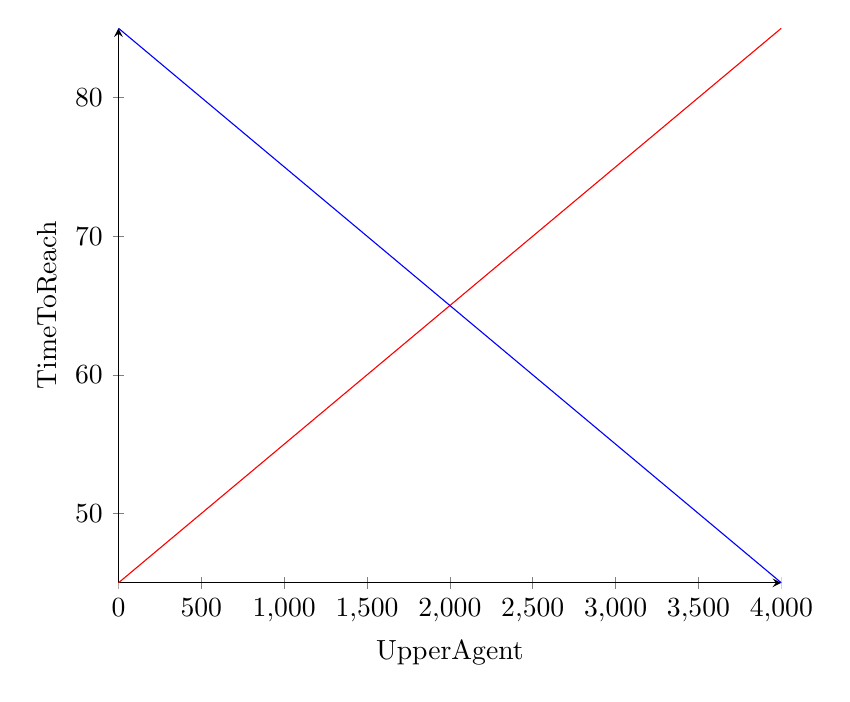
\begin{tikzpicture}
\begin{axis}[
    axis lines = left,
    xlabel = UpperAgent,
    ylabel = TimeToReach,
]
%Below the red parabola is defined
\addplot [
    domain=0:4000, 
    samples=100, 
    color=red,
]
{x/100 + 45};
\addplot [
    domain=0:4000, 
    samples=100, 
    color=blue,
]
{85 - x/100};

\end{axis}
\end{tikzpicture}
\end{center}
Red is upper agents and blue is lower agents.\\
The Only Point that two Best-Response meet as on (2000, 2000).

\subexercise
\[
U_{x} = 
     \begin{cases}
      [1].\ \ {x \over 100} + 45 &\quad\text {if x Agent choose Upper}; X \le 4000 \\
      [2].\ \  40 + {k\over 100} &\quad\text{if k Agent from X choose C-D}; K \le X\\
      [3].\ \  45 + {4000 - x + k \over 100} &\quad\text{otherwise}\\ 
     \end{cases}
\]

\begin{equation} \label{eq1}
\begin{split}
K \le X & \Rightarrow  40 + {k\over 100} < {x \over 100} + 45 \Rightarrow [2] < [1] \\
& \Rightarrow \text{Every Agent In Upper Road can decrease the cost by choosing the C-D,}\\ 
K = X & \Rightarrow 45 + {4000 - x + k \over 1000} = 85 > 40 + {k \over 100} \\
& \Rightarrow \text{Every Agent In Lower Road can decrease the cost by choosing the C-D,}\\
& \Rightarrow \text{Eventually All agent choose C-D road and X = K = 4000}
\end{split}
\end{equation}
The Nash happen when all agents take A-C-D-B road and cost is 80.\\
Surprisingly adding a new road with cost 0 moved Nash from 65 to 80.

\exercise
\subexercise 1. (B, R, F) \rightarrow (0, 0, 0)

\subexercise Max(Min(U_1)) \Rightarrow Max([0, -1]) \Rightarrow [0]

\subexercise
\\\\
\begin{center}
\begin{tabular}{ |c|c|c|c| } 
\hline
 & L & R \\
\hline
\multirow T & 4.4, 4.4 & 1.4, 5.4 \\ 
B & 1.4, 5.4 & 2.4, 2.4 \\ 
\hline
\end{tabular}
\end{center}

\subexercise 1. (B, R) \rightarrow (2.4, 2.4)

\exercise

\end{document}
